\section{Overview}
Northport is a monolithic kernel, with some modularity planned for later drivers. The kernel is booted via the limine boot protocol, and begins with some platform specific initialization. After this the clock and scheduler are started, and then the kernel operates as series of \textit{mostly} independent subsystems.

The kernel makes full use of multi-processor systems, and can run with minimal memory requirements.

\subsection{Kernel Subsystems}
\begin{itemize}
    \item Memory: physical memory manager, virtual memory managers, kernel heap.
    \item Tasking: software clock, scheduler, threads and processes.
    \item Hardware abstraction: functionality required from the underlying hardware that cannot be provided by a driver. Things like the IPI mechanism used and interrupt management are handled here.
    \item Filesystems: VFS, and filesystem drivers.
    \item Debugging: logging facilities, built-in graphical terminal.
    \item Hardware discovery: ACPI table parsing, PCI device enumeration, device tree parsing.
    \item Driver and Device management: Loading, starting and stopping drivers in response to system events like hardware discovery.
\end{itemize}

\begin{figure}[h]
\centering
\begin{tikzpicture}
    \node (DriverLayer) [rectangle, draw=black, fill=black!10, minimum height=2cm, minimum width=12cm] at (0, 5) {};
    \node (SupportLayer) [rectangle, draw=black, fill=green!10, minimum height=4cm, minimum width=12cm] at (0, 2) {};
    \node (UserLayer) [rectangle, draw=black, fill=magenta!10, minimum height=3cm, minimum width=12cm] at (0, -1.5) {};
    \node (CoreLayer) [rectangle, draw=black, fill=orange!10, minimum height=3cm, minimum width=8cm] {};
    \node (ArchLayer) [rectangle, draw=black, fill=blue!10, minimum height=1cm, minimum width=1cm] {Architecture layer};

    \node [above= 2mm of ArchLayer] {Core Layer};
    \node (UserLabel) [below= 1.5cm of ArchLayer] {User Layer};
    \node (SupportLabel) [above= 1cm of CoreLayer] {Support Layer};
    \node (DriverLabel) [above= 0.75cm of SupportLayer] {Drivers};

    \node [rectangle, draw=black, fill=gray!10, above right = 3mm of ArchLayer] {PMM};
    \node [rectangle, draw=black, fill=gray!10, right = 6mm of ArchLayer] {VMM};
    \node [rectangle, draw=black, fill=gray!10, below right = 3mm of ArchLayer] {IPC};
    \node [rectangle, draw=black, fill=gray!10, above left = 2mm of ArchLayer] {Scheduler};
    \node [rectangle, draw=black, fill=gray!10, left = of ArchLayer] {VFS};
    \node [rectangle, draw=black, fill=gray!10, below left = 3mm of ArchLayer] {Clock};
    \node [rectangle, draw=black, fill=gray!10, below = 3mm of ArchLayer] {IPI mailboxes};

    \node [rectangle, draw=black, fill=gray!10, left = 3mm of UserLabel] {System Calls};

    \node [rectangle, draw=black, fill=gray!10, left = 3mm of SupportLabel] {Process management};
    \node [rectangle, draw=black, fill=gray!10, above left = 2mm of SupportLabel] {Debug Terminal};
    \node [rectangle, draw=black, fill=gray!10, below left = 3mm of SupportLabel] {Logging};
    \node [rectangle, draw=black, fill=gray!10, above right = 2mm of SupportLabel] {hardware detect};
\end{tikzpicture}
\end{figure}

There are some other minor subsystems like interrupt vector allocation and IPI mailboxes for communicating on multi-core systems.

\subsection{Init Sequence}
The philosophy of the entry sequence for the kernel is to allow the platform core to contain the messy parts required to interface with hardware, and call various hooks for generic parts of the init sequence when appropriate for the platform. Each architecture contains a \verb|arch/xyz/Init.cpp| file with a few common functions. These functions are not required, but are named this way for consistency.

\begin{itemize}
    \item \verb|KernelEntry()|: This is where the first core starts executing the kernel. This function is usually the ELF entry point, unless the limine boot shim is active. This function does any early set up the platform might require, and then enables the memory subsystems, early platform subsystems (logging), timing subsystem and then performs any core-local set up for BSP (a term borrowed from x86). 
    \item \verb|ApEntry()|: APs (borrowed from x86) require a different codepath to the BSP, and this function is where they begin executing. Most of the time this is just calling \verb|InitCore()|.
    \item \verb|InitCore()|: This function is either called by \verb|KernelEntry()| or \verb|ApEntry()| and performs any initialization required for each processor core in the system. This includes allocating and populating the core-local block, and setting any supported feature flags.
\end{itemize}

\subsubsection{Platform-Independent Init}
The file \verb|CommonInit.cpp| contains initialization code that needs to happen across all platforms. These are provided as hooks that the platform-specific init code can call when it's ready. These hook functions should be called in order.

\begin{itemize}
    \item \verb|InitEarlyPlatform()|: This should be called as early as possible. Here bootloader data is verified to be sane, and the HHDM base and length are determined. Early outputs for logging are detected here, namely a bootloader-provided framebuffer and serial devices.
    \item \verb|InitMemory()|: Initializes the physical memory manager, virtual memory manager and the kernel heap.
    \item \verb|InitPlatform()|: Hardware discovery methods are initialized here (ACPI tables and/or the DTB are parsed). Some global kernel state is also initialized like the core-independent part of the scheduler and interrupt vector allocator.
    \item \verb|ExitBspInit()|: Starts the system clock and then calls \verb|ExitApInit()| (see below).
    \item \verb|ExitApInit()|: Sets up the IPI mailbox for the core, decreases a reference count to bootloader data and then begins scheduled execution. If the reference count is decremented to 0, the core will launch a thread that reclaims bootloader memory and makes it available to the physical memory manager.
\end{itemize}

\begin{figure}[h]
\begin{tikzpicture}
    \node (ApEntry) [rectangle, minimum height=1.5cm, draw=black, fill=blue!10] {
        \verb|ApEntry()|};
    \node (KernelEntry) [rectangle, minimum height=1.5cm, draw=black, fill=blue!10, below = of ApEntry] {
        \verb|KernelEntry()|};
    \node (hidden) [left = 2cm of KernelEntry] {};
    \node (InitCore) [rectangle, minimum height=1.5cm, draw=black, fill=blue!10, right = 3mm of ApEntry] {
        \verb|InitCore()|};
    \node (SchedulerExec) [rectangle, minimum height=1.5cm, draw=black, fill=gray!10, right = of InitCore] {
        Scheduled execution
    };
    \node (InitEarlyPlatform) [rectangle, minimum height=1.5cm, draw=black, fill=gray!10, below = of KernelEntry] {
        \verb|InitEarlyPlatform()|};
    \node (InitMemory) [rectangle, minimum height=1.5cm, draw=black, fill=gray!10, right = 3mm of InitEarlyPlatform] {
        \verb|InitMemory()|};
    \node (InitPlatform) [rectangle, minimum height=1.5cm, draw=black, fill=gray!10, right = 3mm of InitMemory] {
    \verb|InitPlatform()|};

    \path [->, red, dashed] (hidden) edge (KernelEntry.west) node [label=above:Bootloader exit]{};
    \path [->] (KernelEntry.south) edge (InitEarlyPlatform);
    \path [->, in=150, out=-30] (KernelEntry.south) edge (InitMemory.north);
    \path [->, in=140, out=-10] (KernelEntry.south) edge (InitPlatform.north);
    \path [->, red, dashed] (KernelEntry) edge (ApEntry);
    \path [->, bend right, blue!80] (KernelEntry) edge (InitCore);
    \path [->, blue!80] (ApEntry) edge (InitCore);
    \path [->] (InitCore) edge (SchedulerExec);
\end{tikzpicture}

\centering
\begin{tabular}{c|c|l}
    \begin{tikzpicture}
        \path [->, red, dashed] (0, 0) edge (1, 0);
    \end{tikzpicture} 
    & 
    & Platform-specific mechanism. \\

    \begin{tikzpicture}
        \path [->, blue!80] (0, 0) edge (1, 0);
    \end{tikzpicture} 
    & 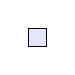
\begin{tikzpicture} \node (r)[rectangle, draw=black, fill=blue!10] (0, 0){}; \end{tikzpicture} 
    & (Call to) platform specific code. \\

    \begin{tikzpicture}
        \path [->, black] (0, 0) edge (1, 0);
    \end{tikzpicture} 
    & 
\begin{tikzpicture} \node (r)[rectangle, draw=black, fill=gray!10] (0, 0){}; \end{tikzpicture}
    & (Call to) common init code. \\
\end{tabular}
\caption{Kernel operation pre-scheduler.}
\end{figure}

\subsection{Multi-Core Systems}
The kernel is written and tested with multi-core systems in mind, but it's also capable of running on single-core systems. 

From the perspective of the kernel, each core is independent. This means any available processor extensions are detected per-core, and the kernel has full support for heterogenous core setups.

Most kernel subsystems operate without knowing how many cores are present in a system, with notable exceptions being the scheduler (\autoref{Scheduler}) and IPI mailboxes. The kernel heap (\autoref{Heap}) can optionally use core-local caches to speed up allocation and reduce a common source of contention between cores.

During early initalization, one core is brought online first and is referred to as the BSP (a term borrowed from x86). The BSP does some initial memory management setup and enable any early log outputs before bringing up the cores. At this point each core will initialize itself, detecting and enabling any extensions. One this is done each core then begins processing work from the scheduler.

Once scheduled execution has begun, the cores are treated mostly equally with the exception of timekeeping. One core (usually the BSP, but it's not required to be) is nominated to manage the software clock (\autoref{Clock}), ensuring clock events have their callbacks called at the correct time and on the correct processor. This core also becomes responsible for managing the hardware timers used to manage the clock.

If for some reason a function is required to run on a specific core, there are two options:
\begin{itemize}
    \item A thread can be created to run the function, and pinned to a specific core. This is the recommended approach for code without timing requirements.
    \item Each core has an IPI mailbox. Each mail item consists of a function pointer and an argument to pass to the function when run. When mail is sent the target core is sent an IPI and the function will whenever the IPI is served. See the function \verb|SendIpiMail()| in \verb|interrupts/Ipi.h|.
\end{itemize}

\subsubsection{Example Code}
To use the mailbox mechanism all that's required a pointer to the function to run on the remote core. In the example we'll assume core 5 exists and we want to run \verb|ExampleFunction()| on that core. The callback function can optionally have an argument passed to it at runtime, but it's not required so we'll use \verb|nullptr|. We omit the argument in this example. The function we'll use is defined in \verb|interrupts/Ipi.h|.

\begin{lstlisting}
void ExampleFunction(void* ignored);

SendIpiMail(5, ExampleFunction, nullptr);
\end{lstlisting}
